\documentclass[10pt,twocolumn]{article}
\usepackage[margin=2.3cm]{geometry}
\usepackage{float}
\restylefloat{table}
\usepackage{cite}
\usepackage{hyperref}
\usepackage{graphicx}
\usepackage{authblk}
\usepackage[latin1]{inputenc}
\usepackage{subfigure}
\usepackage{listings}
\usepackage{float}
\usepackage{fancyvrb}
\usepackage{multirow}
\usepackage{changebar}
%\usepackage{url}
\usepackage{array}
\usepackage{color}
\usepackage{rotating}
\usepackage{titlesec}
\restylefloat{figure}
\usepackage{epstopdf}
\usepackage{colortbl}
\usepackage{setspace}
%\usepackage{breakurl}
\usepackage[belowskip=-5pt]{caption}
\singlespacing
\usepackage{amsmath}
\usepackage{amssymb}

\newcommand{\attGood}{\ensuremath{\checkmark}}
\newcommand{\attBad}{\ensuremath{\times}}


\begin{document}
\title{{\bf Optimizing Latency and Throughput Trade-offs in a Stream Processing System}}
\author[1]{{Joao Carreira, Jian Neng Li}}
%\date{October 2014}
\date{}
\maketitle

%%%%%%%%%%%%%%%%%%%%%%%%%%%%%%%%%%%%%%%%%%%%%%
%\begin{abstract}
%\noindent
%\noindent Large-scale data processing systems such as Spark and Hadoop MapReduce were developed for clusters built on commodity hardware. In this paper, we argue that current market trends invalidate some of the assumptions made by those systems, and we should therefore revisit the designs and architectures derived from them. For example, newer technologies including InfiniBand offer faster network connectivity, and advances in SSDs continue to drive down the cost of fast non-volatile memory. One new architecture that explores these new technologies is Firebox, a hardware building block for future Warehouse-Scale Computers (WSCs). We use Firebox in our studies, and evaluate the behavior changes of large-scale systems under the new settings. In particular, we measure the performance of Spark and applications in the Spark ecosystem under specific workloads, and critique the validity of its underlying assumptions and design decisions.

%\end{abstract}

%\vfill
%\eject
%%%%%%%%%%%%%%%%%%%%%%%%%%%%%%%%%%%%%%%%%%%%%%
\section{Introduction}
\noindent

Many data analytics applications, like intrusion detection and web search, require the computation of results in a timely fashion in order to provide interactivity and fast response to incoming events.
Data analytics systems like Storm~\cite{Storm} or Spark Streaming~\cite{SparkStreaming} provide easy-to-use and deploy frameworks for these types of applications. Storm handles data by creating pipelines for record-at-a-time processing with at-least-once semantics.Spark Streaming offers processing capabilities with micro-batches, where records are coalesced into small groups before being consumed together.
Spark Streaming 


Spark Streaming is stream processing engine built on top of Spark, a fast and general-purpose engine for large-scale data processing. It implements the discretized stream (D-Stream) abstraction, and uses a micro-batch approach to process data as they are received. The application specifies the number of receivers and a batch interval, and Spark Streaming will process all of the data received in the interval by all receivers in a continuous, batched fashion. Every batch job is divided into map and reduce stages, each of which contains tasks that need to be scheduled. Internally, a variable called block interval controls the period of time before a receiver generates a new block. The total number of blocks generated in a batch interval corresponds to the number of tasks spawned for every stage of the resulting batch job.

We perform an in-depth analysis of Spark Streaming, and introduce a number of improvements to the system so that it can handle applications with latency requirements on the order of hundreds or even tens of milliseconds while sacrificing as little as possible on throughput. More specifically, we focus on three main areas of improvements. The first area is to reduce the overhead of running tasks. As tasks are executed, there are a number of inefficiencies in terms of sending duplicate data and performing redundant computations. The second area is the scheduling scalability. Currently, Spark uses a centralized scheduler, which becomes a bottleneck as the number of tasks needed to be scheduled increases with the increase in number of receivers or decrease in the block interval. The third area of focus is the network overhead. The amount of network communication is proportional to the number of tasks running concurrently. We propose an enhancement that uses newer technology such as InfiniBand to reduce the transmission delay, or remote direct memory access (RDMA) to relieve the burden of sending and receiving network packets from the driver CPU.

The paper is organized as follows: in Section 2 we motivate the importance of solving the problem of high task overhead and limited scheduling scalability. In Section 3 we propose measures and techniques to solve these problems. An evaluation of this work is presented in Section 4. Finally, we conclude in Section 5.



\section{Motivation}
\subsection{Task Overheads}
Since tasks form the basic units of computation for Spark Streaming (NOTE: the problem is that tasks are short), it is important to optimize its execution. 
As the system is still relatively new, much of the current codebase emphasizes more on the ease of understanding over raw performance. By analyzing the decisions made by the developers and measuring execution times in different sections of the code path, we found a number of inefficiencies that can be improved upon.

For every Spark Streaming application, there is a driver and multiple executors. The receivers of data run on executors, and these receivers send to the driver metadata about the blocks generated. After every batch interval, the driver collects all of the blocks received during the period and make them into a RDD, and runs application logic on it using Spark. Spark runs each function on the RDD by generating tasks, serialize them, and send them to appropriate executors. The executors deserialize each task, runs the function, and returns to the driver the results.

During our experiments, we found that when a task is not computation-intensive, the majority of the time in running the task is spent in deserialization. When running tasks with no-op operations, we found that from the driver's perspective, the time it takes for a task to be scheduled to the time it takes for the result to be received is 5ms. However, approximately 3.6ms out of this time is spent deserializing the task. These metrics mean that if we can reduce the task deserialization time, there will be a considerable improvement to the latency of small tasks.


\subsection{Scheduling Scalability}

During the execution of a Spark Streaming application, the Driver (a central component of Spark) generates tasks periodically and adds them to the tail of a scheduling queue. This queue is continuously probed by the scheduler which takes tasks from the queue and sends them to worker nodes for processing -- scheduling.
As the tasks get smaller, driven by the need to deliver results as quickly as possible, and become more frequently generated, the number of tasks added to the queue per unit of time increases. If enough tasks per second are generated, the scheduler is not able to keep up with the rate of tasks being added to the queue. This results in tasks starting to queue up and the average time to schedule a task increases indefinitely.

We have benchmarked the latency (end-to-end time to completion) of Spark Streaming tasks with different batch intervals. Lower batch intervals lead to lower task latencies, less throughput and more tasks scheduled per second. On the other hand, larger batch intervals lead to higher throughput, higher task latencies and less tasks scheduled per second. Our benchmark (see graph X)  




\section{Implementation}
\subsection{Task overheads}
Having discovered that a significant portion of the time spent running small tasks is in deserialization, we further measured the time it took individual components of deserialization to complete. Figure \ref{fig:deserialization} summarizes the workflow of task deserialization on the executor. An array of bytes called $serializedTask$ is deserialized into a tuple of $taskFiles$, $taskJars$, and $taskBytes$, the first two of which are passed into a method called $updateDependencies()$, while the latter is further deserialized into a $Task$ object. The $Task$ object contains information such as the function to run, the RDD to use, and the partition of the RDD to operate on.


What we found is that in order to reduce the amount of duplicate data transferred, Spark 1.1.0 wraps the function and the RDD into a broadcast variable. This way, each executor will only fetch the function and the RDD of a batch once. The first task that uses the information will pull it from the driver, and cache the result within the executor for later tasks. In the Spark Streaming context however, this means for every stage, some task on every executor requires a round trip to the driver to fetch the broadcast variable, increasing the latency. As the batch interval shrinks, new RDDs are created more often, but the functions to operate on them do not change. The executor should be able to cache them for a longer period of time than only for the current stage. We have reverted the implementation to not use the broadcast variable, and have already seen latency improvements when the number of executors is relatively small. We plan to further optimize this part by caching functions across stages.

Another interesting discovery regarding the deserialization time is that in $updateDependencies()$, the current implementation creates a new Hadoop configuration object regardless of whether new dependencies are introduced. However, this objection creation is very costly in CPU cycles. We have changed the object to be lazily instantiated, and are seeing an order of magnitude improvement in the execution time of that function.


\subsection{Scheduling Scalability}


To enable a higher scheduling rate of tasks by Spark Streaming, we propose to 1) schedule all tasks per worker in bulk and 2) physically decouple the scheduling (Scheduler) of tasks from their generation (Driver).
First, at each scheduling stage, instead of sending multiple tasks for each node separately, we coalesce them into the same message. This reduces the serialization and networking overheads that result from sending many small messages.
Secondly, as the task generation rate surpasses the scheduling rate, the driver elastically spawns schedulers in remote physical nodes. Thereafter, tasks are forwarded, according to some policy, to these newly spawned schedulers for scheduling (see Figure \ref{fig:schedarch}). 

We have implemented this decentralized architecture in Spark Streaming. Due to the instability of connections between the schedulers, the driver and the workers -- connections are dropped after running the system for a few minutes -- we are currently not able to evaluate the performance benefits of this technique. We plan to fix this engineering problem and report on further results.

\subsection{Network Overhead}
We plan to look into the proposed solutions in this area next.


\section{Related Work}
\team{May be a good idea to push this to the beginning of the paper to show that not everything we are doing has been done before. Perhaps after motivation}

\paragraph {\bf Scheduling} Scheduling papers (policies, scalability, low-latency) go here~\cite{Sparrow}

\paragraph {\bf Streaming} Streaming systems go here. A big portion of these are not low-latency. Those that are better have some limitation that Spark Streaming does not.

\paragraph {\bf Something more databases oriented, e.g., dataflows?}

\paragraph {\bf Approximate Query Engines} Past work \cite{BlinkDB, OnlineAggregation} has focused on providing statistically accurate answers to reduce the computation time and achieve fast response times. Our techniques focus instead on reducing the overheads of analytics systems.




\section{Conclusion}
\noindent

\begin{figure}[t!]
  \begin{center}
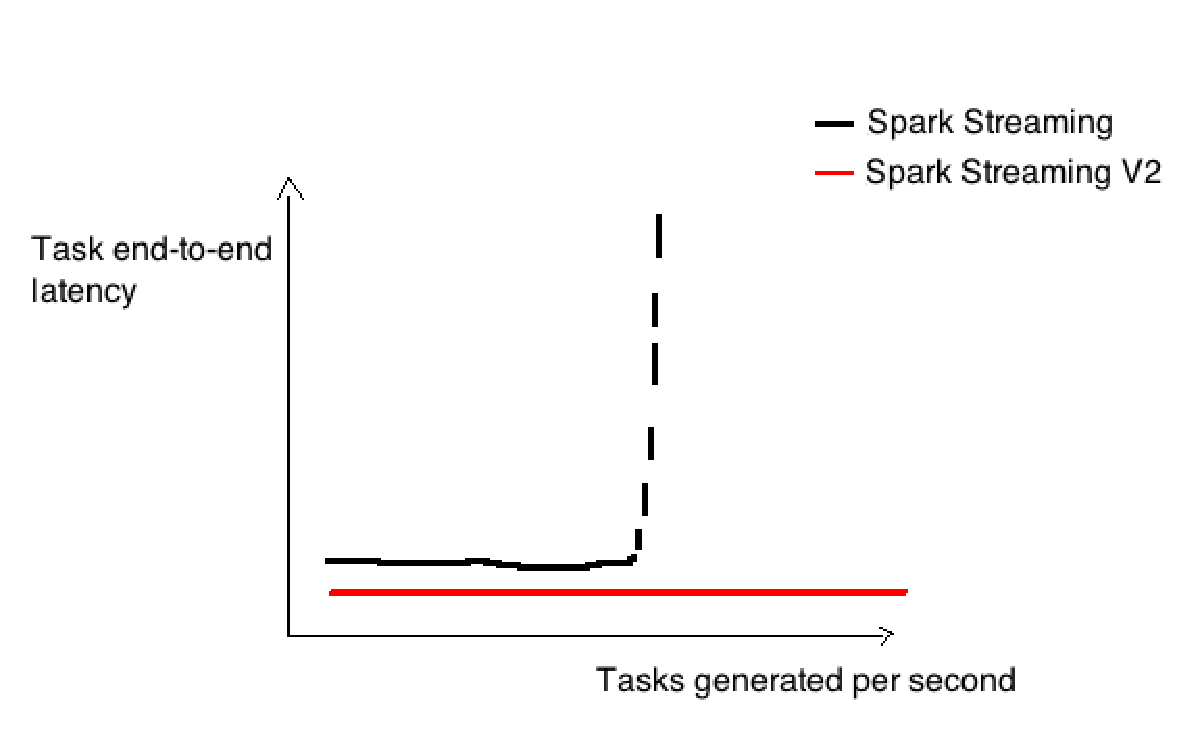
\includegraphics[scale=0.4]{money_graph.eps}
  \end{center}
  \caption{End-to-end latency of individual tasks for varying task generation rates. Improvement results of our proposed techniques.}
  \label{fig:money_graph}
\end{figure}

This paper tries to present a solution for stream processing of short tasks in Spark Streaming - a space that we have found Spark Streaming lacking in practice.
We present three techniques to achieve this goal: 1) reduction of task overheads, 2) decentralized and elastic scheduling, and 3) leveraging modern network mediums of communication for faster transfer of data between the driver, schedulers and workers.

Much of this work is still in progress. We plan to continue working on this problem and evaluating the solutions we have proposed. Figure~\ref{fig:money_graph} shows the result we want to obtain with the techniques we have proposed. We expect the average end-to-end latency of tasks to be lower and the scheduling "capacity" to be higher and a function of the available hardware resources.


%%%%%%%%%%%%%%%%%%%%%%%%%%%%%%%%%%%%%%%%%%%%%%%%%%%%%%%%%%%%%%%%%%%%%%%%%%%%%%%%
% \pagebreak
\bibliography{main}
\bibliographystyle{abbrv}

\end{document}
